\documentclass[11pt, a4paper]{report}
\usepackage[utf8]{inputenc}
\usepackage{pgfplots}

\usepackage[top=2cm, bottom=2.3cm, left=2cm, right=2cm]{geometry}

\title{Graficos das geracoes do NSGA2}
\author{Douglas Nunes de Oliveira}
\date{November 2021}


\begin{document}
    \begin{center}
        \textbf{Utilizando o NSGA2 para o problema DTLZ1.}
        
        \textbf{Gráficos do espaço dos objetivos nas gerações ``1, 20, 40, 60, 80, 100 e 1000''}
        
        
    \end{center}
    

    \begin{center}
    \textbf{Geração 1}
\end{center}

\begin{figure}[h]
    \centering
    \label{fig:geracao01}
    
    \begin{tabular}{rl}
        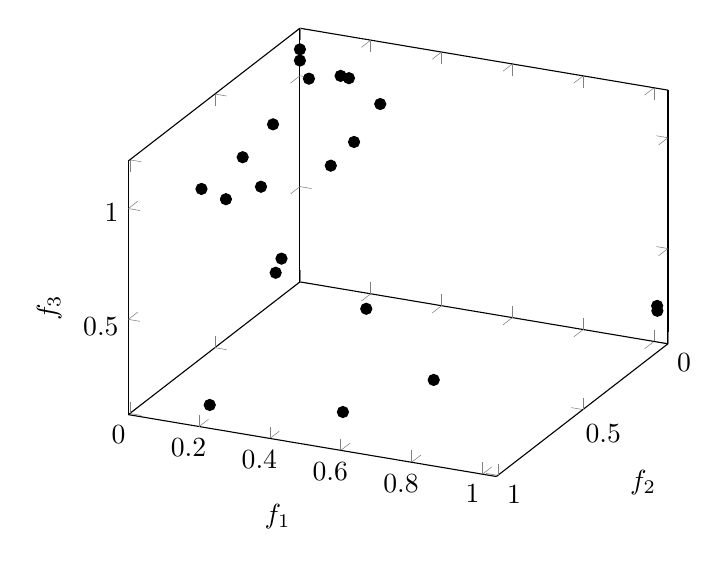
\begin{tikzpicture}[scale=1.0]
        	\begin{axis}[xlabel=$f_2$, ylabel=$f_1$, zlabel=$f_3$, view/h=115]
    			
    			\addplot3[only marks] coordinates {
            		(0.898985, 0.553341, 0.165563) (1.008660, 0.229953, 0.175532) (0.062171, 1.039330, 0.255872) (0.000000, 0.000000, 1.068948) (0.000000, 0.000000, 1.119406) (0.813499, 0.578235, 0.587300) (0.055647, 1.035543, 0.273132) (0.709822, 0.718883, 0.242456) (0.776314, 0.304513, 0.654200) (0.586016, 0.072568, 0.810780) (0.694715, 0.281731, 0.663309) (0.263698, 0.279511, 0.933176) (0.523794, 0.141747, 0.848635) (0.095871, 0.071497, 1.063344) (0.378926, 0.269237, 0.891967) (0.625020, 0.022316, 0.866778) (0.022923, 0.149424, 1.043225) (0.435767, 0.047729, 0.904337) (0.295924, 0.066268, 0.974661) (0.023673, 0.126287, 1.047775) (0.047674, 0.249717, 0.968201) 


        		};
        	\end{axis}
	    \end{tikzpicture}
	    &
	    \begin{tikzpicture}[scale=1.0]
        	\begin{axis}[xlabel=$f_2$, ylabel=$f_1$, zlabel=$f_3$, view={45}{0}]
    			
    			\addplot3[only marks] coordinates {
            		(0.198659,1.402927,0.030436)(0.243016,1.009920,0.490406)(0.965942,0.316067,0.944104)(0.926777,1.057248,0.066572)(0.755361,1.454336,0.018711)(1.099215,0.001117,0.701296)(0.930406,0.386454,0.145874)(0.363359,0.141019,1.073644)(0.005555,0.002258,1.133576)(1.244191,0.475865,0.000000)(0.055722,1.206260,0.087339)(0.122153,0.960673,0.791197)(1.197703,0.000000,0.012183)(0.338440,0.645361,1.002919)(1.231961,0.176431,0.126477)(0.842002,1.466963,0.128832)(1.400163,0.069214,0.140365)(0.050612,0.297072,1.183874)(0.177113,0.032273,1.369730)(0.096804,0.169118,1.443461)(1.185475,0.441860,0.309690) 

        		};
        	\end{axis}
	    \end{tikzpicture}
	\end{tabular}
    
\end{figure}


    \hrulefill
    \begin{center}
    \textbf{Geração 20}
\end{center}

\begin{figure}[h]
    \centering
    \label{fig:geracao01}
    
    \begin{tabular}{rl}
        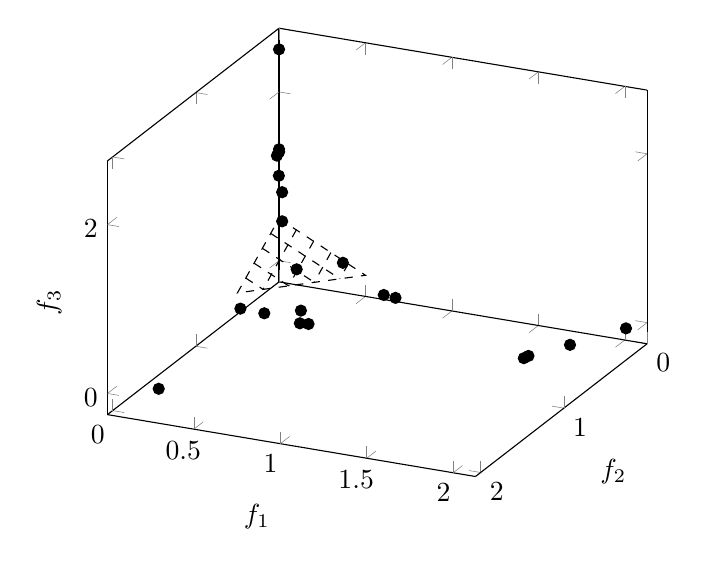
\begin{tikzpicture}[scale=1.0]
        	\begin{axis}[xlabel=$f_2$, ylabel=$f_1$, zlabel=$f_3$, view/h=115]
        		
    			\addplot3[style={dashed}]coordinates {
    			    (0., 0., 0.5) (0., 0.5, 0.) (0.5, 0., 0.) (0., 0., 0.5)
    			};
    			
    			\addplot3[style={dashed}]coordinates {(0., 0.1, 0.4) (0.4, 0.1, 0.)};
    			\addplot3[style={dashed}]coordinates {(0., 0.2, 0.3) (0.3, 0.2, 0.)};
    			\addplot3[style={dashed}]coordinates {(0., 0.3, 0.2) (0.2, 0.3, 0.)};
    			\addplot3[style={dashed}]coordinates {(0., 0.4, 0.1) (0.1, 0.4, 0.)};
    			
    			\addplot3[style={dashed}]coordinates {(0.4, 0., 0.1) (0.4, 0.1, 0.)};
    			\addplot3[style={dashed}]coordinates {(0.3, 0., 0.2) (0.3, 0.2, 0.)};
    			\addplot3[style={dashed}]coordinates {(0.2, 0., 0.3) (0.2, 0.3, 0.)};
    			\addplot3[style={dashed}]coordinates {(0.1, 0., 0.4) (0.1, 0.4, 0.)};
    			
    			\addplot3[only marks] coordinates {
            		(0.196283, 0.196542, 0.115822) (0.269935, 0.735743, 0.053505) (0.031118, 0.033150, 0.502100) (0.752572, 0.276971, 0.046618) (0.003142, 0.002071, 1.292353) (0.280071, 0.808486, 0.052340) (0.589592, 0.410344, 0.000000) (0.806199, 0.164489, 0.103897) (0.000000, 0.000000, 1.320581) (0.008603, 0.003156, 1.014277) (0.753674, 0.483285, 0.000000) (0.253436, 2.128926, 0.125329) (2.062402, 0.296612, 0.157661) (0.000000, 0.000000, 2.503756) (0.732450, 1.768525, 0.013297) (0.745924, 0.529591, 0.001966) (0.046693, 0.010191, 1.284135) (0.253247, 0.491248, 0.337914) (0.613106, 1.978224, 0.152563) (0.101142, 0.066559, 0.911879) (0.712078, 1.785529, 0.030495) 

        		};
        	\end{axis}
	    \end{tikzpicture}
	    &
	    \begin{tikzpicture}[scale=1.0]
        	\begin{axis}[xlabel=$f_2$, ylabel=$f_1$, zlabel=$f_3$, view={45}{0}]
        		
    			\addplot3[style={dashed}]coordinates {
    			    (0., 0., 0.5) (0., 0.5, 0.) (0.5, 0., 0.) (0., 0., 0.5)
    			};
    			
    			\addplot3[only marks] coordinates {
            		(0.000000,0.000000,87.300037)(4.840861,33.459786,20.638485)(48.422177,0.000000,9.858856)(13.120383,31.549160,8.622943)(26.342093,16.373493,6.107313)(0.000000,52.412139,0.000000)(15.055247,28.814203,0.000000)(47.918982,0.001228,9.892156)(51.849355,0.000000,0.000000)(0.000000,0.000000,129.032158)(7.270213,37.696192,24.202731)(44.114677,27.665288,37.262087)(0.000000,92.055748,0.000000)(18.624360,39.312601,2.697538)(53.270066,0.236501,0.000000)(54.632352,0.000000,0.000000)(52.023415,34.357004,0.000000)(159.417210,0.000000,0.000000)(0.000000,168.581518,0.000000)(0.000000,0.000000,130.023145)(60.085897,28.951911,46.264353)

        		};
        	\end{axis}
	    \end{tikzpicture}
	\end{tabular}
    
\end{figure}



    \newpage

    \begin{center}
    \textbf{Geração 40}
\end{center}

\begin{figure}[h]
    \centering
    \label{fig:geracao01}
    
    \begin{tabular}{rl}
        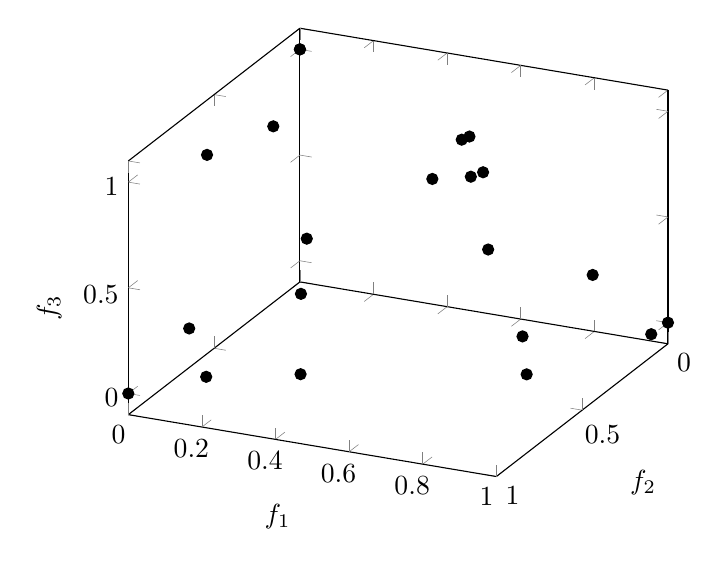
\begin{tikzpicture}[scale=1.0]
        	\begin{axis}[xlabel=$f_2$, ylabel=$f_1$, zlabel=$f_3$, view/h=115]
    			\addplot3[only marks] coordinates {
            		(1.000000, 0.000000, 0.000000) (0.000000, 1.000005, 0.000000) (0.541310, 0.000000, 0.840826) (0.000000, 0.000000, 1.000000) (0.000000, 0.000000, 1.000100) (0.690770, 0.340668, 0.638039) (0.440888, 0.717065, 0.540097) (0.283763, 0.596710, 0.750610) (0.972652, 0.198867, 0.120003) (0.503432, 0.839569, 0.204175) (0.804128, 0.377736, 0.459023) (0.392292, 0.110508, 0.914662) (0.174991, 0.521211, 0.835300) (0.361131, 0.528193, 0.768503) (0.088933, 0.996042, 0.000000) (0.940498, 0.137695, 0.310651) (0.515189, 0.856284, 0.036855) (0.245252, 0.612009, 0.751863) (0.238386, 0.906635, 0.348119) (0.147666, 0.529444, 0.835399) (0.895597, 0.419339, 0.148531) 

        		};
        	\end{axis}
	    \end{tikzpicture}
	    &
	    \begin{tikzpicture}[scale=1.0]
        	\begin{axis}[xlabel=$f_2$, ylabel=$f_1$, zlabel=$f_3$, view={45}{0}]
    			\addplot3[only marks] coordinates {
            		(1.010984,0.000000,0.000000)(0.000000,1.037529,0.000000)(0.000000,0.000000,1.030206)(0.000000,0.000000,1.074789)(0.665893,0.744773,0.198561)(0.673572,0.401364,0.663685)(0.218021,0.889701,0.405159)(0.513301,0.088910,0.923083)(0.957956,0.134562,0.265313)(0.079043,1.020902,0.040988)(0.393249,0.981370,0.000000)(0.144434,0.613702,0.831113)(0.842780,0.278098,0.542046)(0.637467,0.308309,0.774694)(0.942479,0.004177,0.474421)(0.838668,0.546414,0.168372)(0.070071,0.673875,0.775207)(0.308683,0.940953,0.320588)(0.254647,0.924109,0.389850)(0.764959,0.478170,0.601281)(0.843468,0.511611,0.251668) 

        		};
        	\end{axis}
	    \end{tikzpicture}
	\end{tabular}
    
\end{figure}


    \hrulefill
    \begin{center}
    \textbf{Geração 60}
\end{center}

\begin{figure}[h]
    \centering
    \label{fig:geracao01}
    
    \begin{tabular}{rl}
        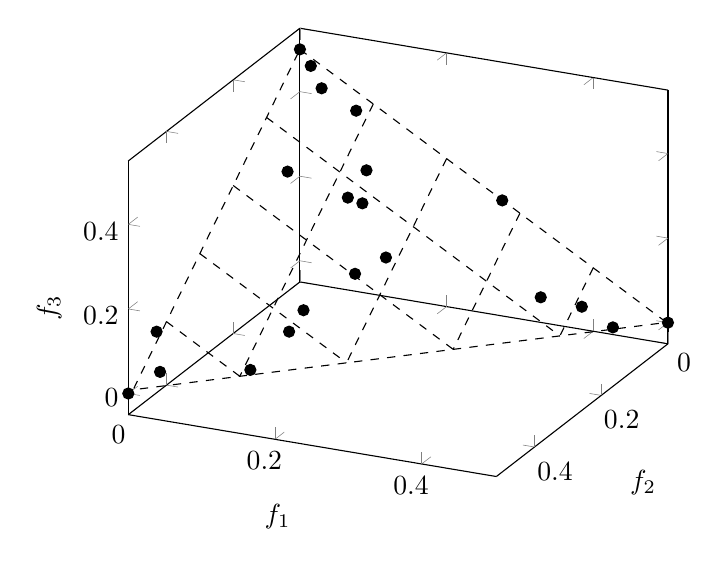
\begin{tikzpicture}[scale=1.0]
        	\begin{axis}[xlabel=$f_2$, ylabel=$f_1$, zlabel=$f_3$, view/h=115]
        		
    			\addplot3[style={dashed}]coordinates {
    			    (0., 0., 0.5) (0., 0.5, 0.) (0.5, 0., 0.) (0., 0., 0.5)
    			};
    			
    			\addplot3[style={dashed}]coordinates {(0., 0.1, 0.4) (0.4, 0.1, 0.)};
    			\addplot3[style={dashed}]coordinates {(0., 0.2, 0.3) (0.3, 0.2, 0.)};
    			\addplot3[style={dashed}]coordinates {(0., 0.3, 0.2) (0.2, 0.3, 0.)};
    			\addplot3[style={dashed}]coordinates {(0., 0.4, 0.1) (0.1, 0.4, 0.)};
    			
    			\addplot3[style={dashed}]coordinates {(0.4, 0., 0.1) (0.4, 0.1, 0.)};
    			\addplot3[style={dashed}]coordinates {(0.3, 0., 0.2) (0.3, 0.2, 0.)};
    			\addplot3[style={dashed}]coordinates {(0.2, 0., 0.3) (0.2, 0.3, 0.)};
    			\addplot3[style={dashed}]coordinates {(0.1, 0., 0.4) (0.1, 0.4, 0.)};
    			
    			\addplot3[only marks] coordinates {
            		(0.514489, 0.000000, 0.000000) (0.000000, 0.501885, 0.000000) (0.000000, 0.000000, 0.500000) (0.075686, 0.362831, 0.065588) (0.001464, 0.276571, 0.224326) (0.049183, 0.449198, 0.003511) (0.052060, 0.408109, 0.042128) (0.314369, 0.128237, 0.061589) (0.279580, 0.132065, 0.092149) (0.471578, 0.023754, 0.031876) (0.082264, 0.128169, 0.301487) (0.387110, 0.108519, 0.009737) (0.020917, 0.086196, 0.392889) (0.155568, 0.188059, 0.157464) (0.429695, 0.000000, 0.094503) (0.198656, 0.165548, 0.138653) (0.028476, 0.042543, 0.437754) (0.121148, 0.120458, 0.258396) (0.013310, 0.020866, 0.475096) (0.141795, 0.047627, 0.311314) (0.116752, 0.138291, 0.247420) 

        		};
        	\end{axis}
	    \end{tikzpicture}
	    &
	    \begin{tikzpicture}[scale=1.0]
        	\begin{axis}[xlabel=$f_2$, ylabel=$f_1$, zlabel=$f_3$, view={45}{0}]
        		
    			\addplot3[style={dashed}]coordinates {
    			    (0., 0., 0.5) (0., 0.5, 0.) (0.5, 0., 0.) (0., 0., 0.5)
    			};
    			
    			\addplot3[only marks] coordinates {
            		(25.557095,0.000000,0.000000)(0.000000,25.862771,0.000000)(0.000000,0.000000,18.808556)(8.145637,16.904257,5.176290)(4.234293,13.764281,11.321800)(20.083563,2.787875,0.000000)(10.906111,5.246635,9.110277)(1.232655,22.097753,1.542088)(3.658022,6.843465,17.676222)(10.750896,0.000000,13.886307)(25.475714,2.287804,0.000000)(2.141666,20.390651,2.480924)(17.590100,7.235667,0.000000)(0.979315,9.185810,18.204913)(9.215784,18.565221,0.085940)(13.885205,11.800430,4.728499)(12.629969,12.280675,4.141844)(9.407013,5.101432,9.316532)(5.637196,3.829305,12.926649)(14.849740,6.523113,0.012551)(6.155661,12.330586,11.663643) 

        		};
        	\end{axis}
	    \end{tikzpicture}
	\end{tabular}
    
\end{figure}


    
    \newpage
    \begin{center}
    \textbf{Geração 80}
\end{center}

\begin{figure}[h]
    \centering
    \label{fig:geracao01}
    
    \begin{tabular}{rl}
        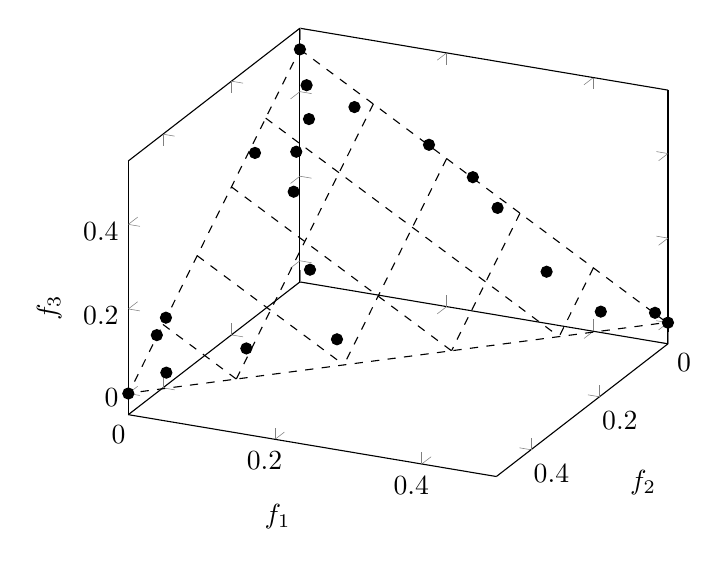
\begin{tikzpicture}[scale=1.0]
        	\begin{axis}[xlabel=$f_2$, ylabel=$f_1$, zlabel=$f_3$, view/h=115]
        		
    			\addplot3[style={dashed}]coordinates {
    			    (0., 0., 0.5) (0., 0.5, 0.) (0.5, 0., 0.) (0., 0., 0.5)
    			};
    			
    			\addplot3[style={dashed}]coordinates {(0., 0.1, 0.4) (0.4, 0.1, 0.)};
    			\addplot3[style={dashed}]coordinates {(0., 0.2, 0.3) (0.3, 0.2, 0.)};
    			\addplot3[style={dashed}]coordinates {(0., 0.3, 0.2) (0.2, 0.3, 0.)};
    			\addplot3[style={dashed}]coordinates {(0., 0.4, 0.1) (0.1, 0.4, 0.)};
    			
    			\addplot3[style={dashed}]coordinates {(0.4, 0., 0.1) (0.4, 0.1, 0.)};
    			\addplot3[style={dashed}]coordinates {(0.3, 0., 0.2) (0.3, 0.2, 0.)};
    			\addplot3[style={dashed}]coordinates {(0.2, 0., 0.3) (0.2, 0.3, 0.)};
    			\addplot3[style={dashed}]coordinates {(0.1, 0., 0.4) (0.1, 0.4, 0.)};
    			
    			\addplot3[only marks] coordinates {
            		(0.501151, 0.000000, 0.000000) (0.000000, 0.501703, 0.000000) (0.000000, 0.000000, 0.500000) (0.041065, 0.355436, 0.103501) (0.000000, 0.235731, 0.266484) (0.156883, 0.064729, 0.280477) (0.359699, 0.094880, 0.045671) (0.013573, 0.275784, 0.214028) (0.000000, 0.175953, 0.325635) (0.040601, 0.429121, 0.030327) (0.066853, 0.043557, 0.389739) (0.279764, 0.181108, 0.042364) (0.449474, 0.027700, 0.025058) (0.112049, 0.047329, 0.341871) (0.145954, 0.006854, 0.348487) (0.018172, 0.082838, 0.399070) (0.226296, 0.119396, 0.155472) (0.417883, 0.000000, 0.085942) (0.391287, 0.000000, 0.110476) (0.035204, 0.025521, 0.444716) (0.000000, 0.484058, 0.018173) 

        		};
        	\end{axis}
	    \end{tikzpicture}
	    &
	    \begin{tikzpicture}[scale=1.0]
        	\begin{axis}[xlabel=$f_2$, ylabel=$f_1$, zlabel=$f_3$, view={45}{0}]
        		
    			\addplot3[style={dashed}]coordinates {
    			    (0., 0., 0.5) (0., 0.5, 0.) (0.5, 0., 0.) (0., 0., 0.5)
    			};
    			
    			\addplot3[only marks] coordinates {
            		(25.557095,0.000000,0.000000)(0.000000,19.177327,0.000000)(0.000000,0.000000,15.470869)(3.037656,6.672029,8.936816)(15.434954,1.229393,10.661216)(5.637196,3.829305,12.926649)(4.844314,10.655167,7.300313)(0.000000,12.296822,5.636917)(5.882303,14.099157,1.845874)(8.940586,8.204036,2.127804)(1.165727,16.318428,2.120988)(17.011234,2.938357,0.984301)(11.845078,11.870279,0.000000)(8.867463,13.563037,3.473916)(8.149641,17.784455,0.449559)(23.541033,1.906498,0.000000)(10.861441,1.290302,7.988342)(19.352375,1.159940,3.186702)(9.307486,0.776347,14.370748)(1.583821,18.413031,0.418250)(21.011899,1.370938,1.268155) 

        		};
        	\end{axis}
	    \end{tikzpicture}
	\end{tabular}
    
\end{figure}


    \hrulefill
    \begin{center}
    \textbf{Geração 100}
\end{center}

\begin{figure}[h]
    \centering
    \label{fig:geracao01}
    
    \begin{tabular}{rl}
        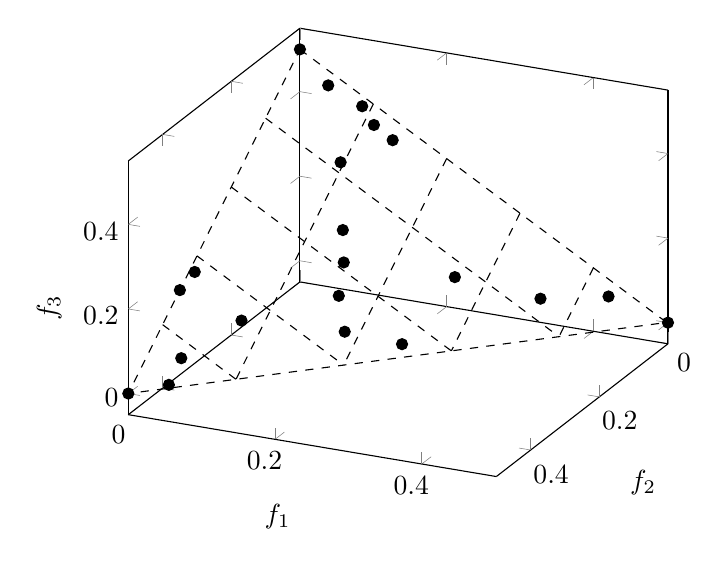
\begin{tikzpicture}[scale=1.0]
        	\begin{axis}[xlabel=$f_2$, ylabel=$f_1$, zlabel=$f_3$, view/h=115]
        		
    			\addplot3[style={dashed}]coordinates {
    			    (0., 0., 0.5) (0., 0.5, 0.) (0.5, 0., 0.) (0., 0., 0.5)
    			};
    			
    			\addplot3[style={dashed}]coordinates {(0., 0.1, 0.4) (0.4, 0.1, 0.)};
    			\addplot3[style={dashed}]coordinates {(0., 0.2, 0.3) (0.3, 0.2, 0.)};
    			\addplot3[style={dashed}]coordinates {(0., 0.3, 0.2) (0.2, 0.3, 0.)};
    			\addplot3[style={dashed}]coordinates {(0., 0.4, 0.1) (0.1, 0.4, 0.)};
    			
    			\addplot3[style={dashed}]coordinates {(0.4, 0., 0.1) (0.4, 0.1, 0.)};
    			\addplot3[style={dashed}]coordinates {(0.3, 0., 0.2) (0.3, 0.2, 0.)};
    			\addplot3[style={dashed}]coordinates {(0.2, 0., 0.3) (0.2, 0.3, 0.)};
    			\addplot3[style={dashed}]coordinates {(0.1, 0., 0.4) (0.1, 0.4, 0.)};
    			
    			\addplot3[only marks] coordinates {
            		(0.500000, 0.000000, 0.000000) (0.000000, 0.501703, 0.000000) (0.000000, 0.000000, 0.500000) (0.157649, 0.132235, 0.210208) (0.087593, 0.096445, 0.316043) (0.015851, 0.045971, 0.438178) (0.421486, 0.035456, 0.044608) (0.264481, 0.184805, 0.052188) (0.119914, 0.267315, 0.114612) (0.022538, 0.111409, 0.367816) (0.019174, 0.429660, 0.052998) (0.318838, 0.005763, 0.175425) (0.074387, 0.362737, 0.062880) (0.011178, 0.090107, 0.398780) (0.231305, 0.161214, 0.109347) (0.191210, 0.149214, 0.159667) (0.349778, 0.000000, 0.150250) (0.459634, 0.036409, 0.005755) (0.334294, 0.076760, 0.090826) (0.232486, 0.247968, 0.021100) (0.024000, 0.137638, 0.340430) 

        		};
        	\end{axis}
	    \end{tikzpicture}
	    &
	    \begin{tikzpicture}[scale=1.0]
        	\begin{axis}[xlabel=$f_2$, ylabel=$f_1$, zlabel=$f_3$, view={45}{0}]
        		
    			\addplot3[style={dashed}]coordinates {
    			    (0., 0., 0.5) (0., 0.5, 0.) (0.5, 0., 0.) (0., 0., 0.5)
    			};
    			
    			\addplot3[only marks] coordinates {
            		(17.814138,0.000000,0.000000)(0.000000,17.643105,0.000000)(0.000000,0.000000,13.977723)(1.601047,10.251867,7.614543)(8.135195,5.670870,2.084032)(1.035720,4.965857,12.009724)(4.364600,12.359378,0.631340)(1.928931,8.790747,6.922857)(6.735992,0.000000,10.180065)(11.212573,0.832881,5.485430)(10.144734,0.000000,6.517945)(15.368517,0.000000,2.597986)(2.658333,6.603699,4.139209)(14.381035,2.091973,0.851876)(0.602773,11.579934,1.417001)(5.429664,5.099744,3.936790)(6.220722,1.214467,10.351246)(3.204461,14.638293,0.000000)(11.832449,0.000000,4.804166)(0.180017,0.101508,13.393921)(2.804775,14.865582,0.000000) 

        		};
        	\end{axis}
	    \end{tikzpicture}
	\end{tabular}
    
\end{figure}


    
    \newpage
    \begin{center}
    \textbf{Geração 1000}
\end{center}

\begin{figure}[h]
    \centering
    \label{fig:geracao01}
    
    \begin{tabular}{rl}
        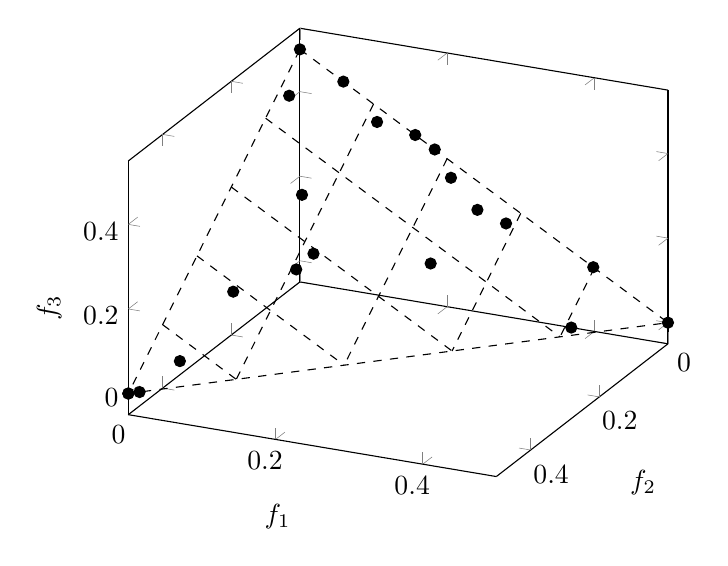
\begin{tikzpicture}[scale=1.0]
        	\begin{axis}[xlabel=$f_2$, ylabel=$f_1$, zlabel=$f_3$, view/h=115]
        		
    			\addplot3[style={dashed}]coordinates {
    			    (0., 0., 0.5) (0., 0.5, 0.) (0.5, 0., 0.) (0., 0., 0.5)
    			};
    			
    			\addplot3[style={dashed}]coordinates {(0., 0.1, 0.4) (0.4, 0.1, 0.)};
    			\addplot3[style={dashed}]coordinates {(0., 0.2, 0.3) (0.3, 0.2, 0.)};
    			\addplot3[style={dashed}]coordinates {(0., 0.3, 0.2) (0.2, 0.3, 0.)};
    			\addplot3[style={dashed}]coordinates {(0., 0.4, 0.1) (0.1, 0.4, 0.)};
    			
    			\addplot3[style={dashed}]coordinates {(0.4, 0., 0.1) (0.4, 0.1, 0.)};
    			\addplot3[style={dashed}]coordinates {(0.3, 0., 0.2) (0.3, 0.2, 0.)};
    			\addplot3[style={dashed}]coordinates {(0.2, 0., 0.3) (0.2, 0.3, 0.)};
    			\addplot3[style={dashed}]coordinates {(0.1, 0., 0.4) (0.1, 0.4, 0.)};
    			
    			\addplot3[only marks] coordinates {
            		(0.500000, 0.000000, 0.000000) (0.500000, 0.000000, 0.000000) (0.000000, 0.500000, 0.000000) (0.000000, 0.000000, 0.500000) (0.022317, 0.290411, 0.187272) (0.000000, 0.398503, 0.101497) (0.309423, 0.053651, 0.136926) (0.152593, 0.073964, 0.273443) (0.236225, 0.105143, 0.158632) (0.000000, 0.156647, 0.343353) (0.000000, 0.183146, 0.316854) (0.016253, 0.112373, 0.371374) (0.425035, 0.035095, 0.039870) (0.057607, 0.012249, 0.430144) (0.030429, 0.255305, 0.214266) (0.017226, 0.213245, 0.269528) (0.205948, 0.114458, 0.179594) (0.081295, 0.406565, 0.012140) (0.124109, 0.235478, 0.140413) (0.489575, 0.010425, 0.000000) (0.000000, 0.058984, 0.441016) 

        		};
        	\end{axis}
	    \end{tikzpicture}
	    &
	    \begin{tikzpicture}[scale=1.0]
        	\begin{axis}[xlabel=$f_2$, ylabel=$f_1$, zlabel=$f_3$, view={45}{0}]
        		
    			\addplot3[style={dashed}]coordinates {
    			    (0., 0., 0.5) (0., 0.5, 0.) (0.5, 0., 0.) (0., 0., 0.5)
    			};
    			
    			\addplot3[only marks] coordinates {
            		(13.026614,0.000000,0.000000)(0.000000,13.026614,0.000000)(0.000000,0.000000,13.026614)(6.607459,2.768464,3.650691)(8.858561,4.168053,0.000000)(4.775350,0.153626,8.097638)(0.038916,3.832737,9.154961)(2.465687,7.841465,2.719462)(0.389702,1.190070,11.446843)(0.019892,10.608245,2.398477)(11.740882,0.905432,0.380301)(10.612149,0.184901,2.229564)(6.328799,0.000000,6.697815)(4.073184,1.682148,7.271282)(1.709631,5.620078,5.696905)(1.920648,6.341865,4.764101)(0.678180,12.348434,0.000000)(0.770733,3.459635,8.796247)(2.439457,7.967100,2.620058)(7.657499,1.655864,3.713251)(3.378821,9.647794,0.000000)

        		};
        	\end{axis}
	    \end{tikzpicture}
	\end{tabular}
    
\end{figure}


    \hrulefill

\end{document}
